\iffalse
\documentclass[12pt]{article}
\usepackage{graphicx}
\usepackage{amsmath}
\usepackage{mathtools}
\usepackage{gensymb}
\usepackage{amssymb}
\usepackage{tikz}
\usetikzlibrary{arrows,shapes,automata,petri,positioning,calc}
\usepackage{hyperref}
\usepackage{tikz}
\usetikzlibrary{matrix,calc}
\usepackage[margin=0.5in]{geometry}

\providecommand{\norm}[1]{\left\lVert#1\right\rVert}
\newcommand{\myvec}[1]{\ensuremath{\begin{pmatrix}#1\end{pmatrix}}}
\let\vec\mathbf
%\providecommand $${\norm}[1]{\left\lVert#1\right\rVert}$$
\providecommand{\abs}[1]{\left\vert#1\right\vert}
\let\vec\mathbf

\newcommand{\mydet}[1]{\ensuremath{\begin{vmatrix}#1\end{vmatrix}}}
\providecommand{\brak}[1]{\ensuremath{\left(#1\right)}}
\providecommand{\lbrak}[1]{\ensuremath{\left(#1\right.}}
\providecommand{\rbrak}[1]{\ensuremath{\left.#1\right)}}
\providecommand{\sbrak}[1]{\ensuremath{{}\left[#1\right]}}

\providecommand{\brak}[1]{\ensuremath{\left(#1\right)}}
\providecommand{\norm}[1]{\left\lVert#1\right\rVert}
\newcommand{\solution}{\noindent \textbf{Solution: }}

\let\vec\mathbf
\def\inputGnumericTable{}
\usepackage{color}                                            %%
    \usepackage{array}                                            %%
    \usepackage{longtable}                                        %%
    \usepackage{calc}                                             %%
    \usepackage{multirow}                                         %%
    \usepackage{hhline}                                           %%
    \usepackage{ifthen}
\usepackage{array}
\usepackage{amsmath}   % for having text in math mode
\usepackage{listings}
\lstset{
language=tex,
frame=single, 
breaklines=true
}
\newenvironment{Figure}
  {\par\medskip\noindent\minipage{\linewidth}}
  {\endminipage\par\medskip}
\begin{document}
\begin{center}
\textbf\large{CLASS-9\\CHAPTER-10 \\ CIRCLES}

\end{center}
\section*{Excercise 10.6}

\section*{\large Solution}:
\fi
The input parameters are available in Table 
	\ref{tab:chapters/9/10/6/1/table1}.
\begin{figure}[H]
\centering
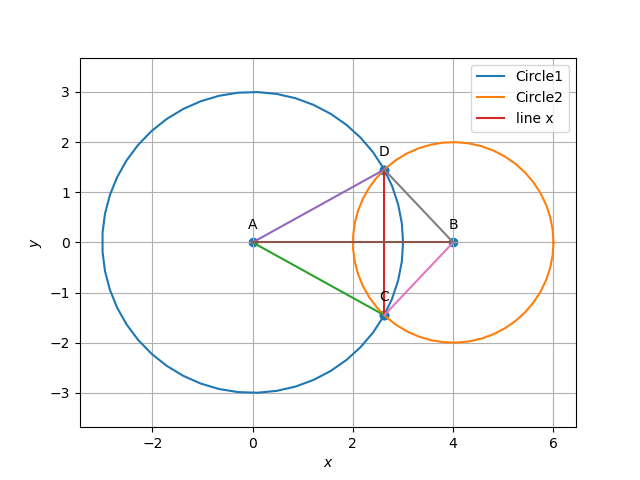
\includegraphics[width=0.75\columnwidth]{chapters/9/10/6/1/figs/circle3.png}
\caption{}
\label{fig:chapters/9/10/6/1/Fig1}
\end{figure}



\begin{table}[H]
	\small
	\centering
	%\subimport{../chapters/9/10/6/1/tables/}{table1.tex}
     \begin{tabular}{|p{3cm}|p{3cm}|p{3cm}|}
\hline                                        
\textbf{Symbol} & \textbf{Values} & \textbf{Description}\\                                          
\hline                                 
$\theta$ & 30$\degree{}$   & $\angle{BAD} = \angle{BAC}$ \\           
\hline                                    
a &  9 & $AB$ \\     
\hline                      
c & 5 & $AC$ \\
\hline                                     
		$\vec{e}_1$ & $\myvec{
			1\\
			0\\
			}$ & basis vector\\ 
\hline
\end{tabular}

%	\caption{}
	\label{tab:chapters/9/10/6/1/table1}
\end{table}
 The two circle equations are given by
\begin{align}
\label{eq:chapters/9/10/6/1/1}
	\norm{x}^2-9&=0\\
	\norm{x}^2-8\vec{e}_1+12&=0
\end{align}
yielding the intersection of the circles as the line
\begin{align}
\myvec{1&0}\vec{x}&=\frac{21}{8}\\
\label{eq:chapters/9/10/6/1/20}
\end{align}
		\eqref{eq:chapters/9/10/6/1/20} can be expressed as
\begin{align}
	\vec{x}=\vec{q}+\lambda\vec{m}\label{eq:chapters/9/10/6/1/21}
\end{align}
The distance form origin to point $\vec{x}$ is given by
\begin{align}
	\norm{\vec{x}}^2&=d^2\label{eq:chapters/9/10/6/1/22}
\end{align}
		Then substituting \eqref{eq:chapters/9/10/6/1/21} in \eqref{eq:chapters/9/10/6/1/22} yeilds,
\begin{align}
	\brak{\vec{q}+\lambda\vec{m}}^{\top}\brak{\vec{q}+\lambda\vec{m}}&=d^2\\
	\implies \lambda^2\norm{\vec{m}}^2+2\lambda\vec{q}^{\top}\vec{m}+\norm{\vec{q}}^2&=d^2\label{eq:chapters/9/10/6/1/26}
\end{align}
where
\begin{align}
	\vec{q}=\myvec{\frac{21}{8}\\0},\vec{m}=\myvec{0\\1} \text{ and } d=r_1=3
	\label{eq:chapters/9/10/6/1/27}
\end{align}
		Substituting the values in \eqref{eq:chapters/9/10/6/1/27} in \eqref{eq:chapters/9/10/6/1/26}, 
\begin{align}
	\lambda^2(1)+2\lambda\myvec{\frac{21}{8}&0}\myvec{0\\1}+\frac{441}{64}&=9\\
	\implies\lambda_i&=\pm\frac{3\sqrt{5}}{8}
\end{align}
Thus, 
the intersecting points $\vec{C}$ and $\vec{D}$ are given by
\begin{align}
    \vec{C}&=\vec{q}+\lambda_1\vec{m}=\myvec{\frac{21}{8}\\[2pt]-\frac{3\sqrt{5}}{8}}\\
    \vec{D}&=\vec{q}+\lambda_2\vec{m}=\myvec{\frac{21}{8}\\[2pt]\frac{3\sqrt{5}}{8}}
\end{align}
\begin{enumerate}
\item Finding $\angle$ADB
	\begin{align}
		 \vec{A-D} = \myvec{-\frac{21}{8}\\[2pt]-\frac{3\sqrt{5}}{8}},
		\vec{B-D}& = \myvec{\frac{11}{8}\\[2pt]-\frac{3\sqrt{5}}{8}}\\
	 \vec{(A-D)^\top(B-D)}&= -\frac{3}{2}\\
	 \norm{\vec{A-D}}\norm{\vec{C-D}}& = 6\\
\implies		\cos(\angle ADB)& = \frac{\vec{(A-D)^\top(B-D)}}{\norm{\vec{A-D}}\norm{\vec{B-D}}}\\
		\text{or, }		\angle ADB&=104\degree
\end{align}
\item Finding $\angle$ACB
\begin{align}
	\vec{A-C} = \myvec{-\frac{21}{8}\\[2pt]\frac{3\sqrt{5}}{8}},
	 \vec{B-C}& = \myvec{\frac{11}{8}\\[2pt]\frac{3\sqrt{5}}{8}}\\
	 \vec{(A-C)^\top(B-C)}&= -\frac{3}{2}\\
	 \norm{\vec{A-C}}\norm{\vec{B-C}}& = 6\\
\implies 	 \cos(\angle ACB) &= \frac{\vec{(A-C)^\top(B-C)}}{\norm{\vec{A-C}}\norm{\vec{B-C}}}\\
	\text{or, }	 \angle ACB&=104\degree = \angle ADB
\end{align}
\end{enumerate}
See Fig. 
\ref{fig:chapters/9/10/6/1/Fig1}.


